% Created 2025-03-07 金 09:30
\documentclass[a4paper, 10pt, notitlepage, uplatex, dvipdfmx]{jsarticle}
\usepackage[dvipdfmx]{graphicx, color}
\usepackage{ulem}
\usepackage[utf8]{inputenc}
\usepackage{mlmodern}
\usepackage{mdframed}
\usepackage{minted}
\usepackage{natbib}
\usepackage{amsmath, amssymb, amsthm}
\definecolor{shadecolor}{gray}{0.92}
\definecolor{bgcode}{gray}{0.98}
\usemintedstyle{friendly}
\usepackage[dvipdfmx,colorlinks=true,linkcolor=blue,filecolor=blue,urlcolor=blue]{hyperref}
\usepackage{pxjahyper}
\surroundwithmdframed[backgroundcolor=shadecolor,hidealllines=true]{verbatim}
\renewcommand{\baselinestretch}{0.9}
\setlength{\voffset}{-0.7in}
\setlength{\topmargin}{-0.5cm}
\setlength{\oddsidemargin}{0cm}
\setlength{\textheight}{45\baselineskip}
\addtolength{\textheight}{\topskip}

\newcommand{\NaID}{\mbox{Na\,{\sc i}\,D}}
\author{sugayu}
\date{\today}
\title{\textbf{orgから\LaTeX{}やHTMLへのエクスポート自分用メモ}}
\begin{document}

\maketitle
\section{org-modeにおける\LaTeX{}文章の書き方}
\label{sec:org5c59a17}
org-exportを使うことでorg文章を\LaTeX{}文章へ変換することができる。
パッケージ名は \texttt{ox-latex} 。

Emacs上における\LaTeX{}クラスは \texttt{init.el} に自分で調整して指定済み。
状況に応じて以下の\LaTeX{}クラスを使いわける。
デフォルトのクラスは1段組みの \texttt{jsarticle} になっている。

\begin{verbatim}
#+LATEX_CLASS: jsarticle2  # 2段組み。長い文章のとき。
#+LATEX_CLASS: jsarticle  # 短い文章や1行が長いとき。
#+LATEX_CLASS: plain-article  # 英文1段組み
\end{verbatim}
クラスのオプションを指定したい場合は以下のようにしてオプションを変更できる。
\begin{verbatim}
#+LATEX_CLASS_OPTIONS: [oneside,twocolumn]
#+LATEX_CLASS_OPTIONS: [a4paper, 9pt, notitlepage, uplatex, dvipdfmx]
\end{verbatim}
デフォルトのコンパイラは \texttt{ptex2pdf -u -l} を使って \texttt{uplatex} を起動させている(はず)。
英文のクラスにする際にはコンパイラを変更する。
\begin{verbatim}
#+LATEX_COMPILER: pdflatex
\end{verbatim}
ヘッダーキーワードは以下のように追加できる。
ここでコマンドを定義すれば \texttt{\textbackslash{}NaID} のようにコマンドを打ったときに \NaID だと\LaTeX{}が認識できる。
ただしHTMLは認識できないので別の方策を考える必要がある。
\begin{verbatim}
#+LATEX_HEADER: \input{template_sub}
#+LATEX_HEADER: \subtitle{2024/09/02--2024/09/08}
\end{verbatim}
これらのヘッダー情報は、他の書類にも共通する内容であれば \texttt{init.el} に書きこんだり \texttt{\textbackslash{}input\{\}} で挿入したりして共通化するのが良い。

他にもorg文書を他の形式へ出力する際の細かな設定は\href{info:org\#Export Settings}{org\#Export Settings}に書かれてある。
例えば、目次(Table of Contents)を表示したくない場合やアンダーバーを下小文字にしたくない場合には以下を打つ。
\begin{verbatim}
#+OPTIONS: toc:nil
#+OPTIONS: ^:nil
\end{verbatim}
\section{要素の挿入}
\label{sec:orga0b5e0c}
\subsection{数式}
\label{sec:org911c88f}
\texttt{org-mode} は\LaTeX{}の数式の仕様を導入してくれているので、そのまま使うことができる。
文章中に数式を挿入すると \(\Sigma_{n = 0}^{\infty} (1/x)^n < 1\ (x = 2)\) のようになる。
数式環境で挿入すると
\begin{equation}
\label{eq:1}
F = \int_{-\infty}^{\infty} f_{\nu} d\nu
\end{equation}
のようになる。
式番号も式\ref{eq:1}のように参照することができる。
このとき \texttt{\#+NAME} を使ってラベルをつける必要があることに注意する。
\subsection{表}
\label{sec:org1726269}
\texttt{org-table} が使える。

\begin{center}
\begin{tabular}{llll}
\hline
\hline
Name & {[}OIII] & {[}NII] & {[}CII]\\
\hline
M82 & \(1\times10^{-22}\) & \(3\times10^{-23}\) & \(1\times10^{-23}\)\\
M101 & \(1\times10^{-22}\) & \(4\times10^{-23}\) & \(1\times10^{-23}\)\\
\hline
\end{tabular}
\end{center}
\subsection{画像}
\label{sec:orgab0471a}
画像は \texttt{org-mode} と同じ要領で入れる。
\texttt{\#+ATTR\_HTML: :width 30\%} を使えばHTML上で各画像のサイズを変更できる。
\texttt{\#+ATTR\_LATEX: :width 0.38\textbackslash{}textwidth} を使えば\LaTeX{}上でサイズを変更できる。
\begin{itemize}
\item \href{info:org\#Images in HTML export}{org\#Images in HTML export}
\item \href{info:org\#Images in LaTeX export}{org\#Images in \LaTeX{} export}
\end{itemize}

\begin{figure}[htbp]
\centering
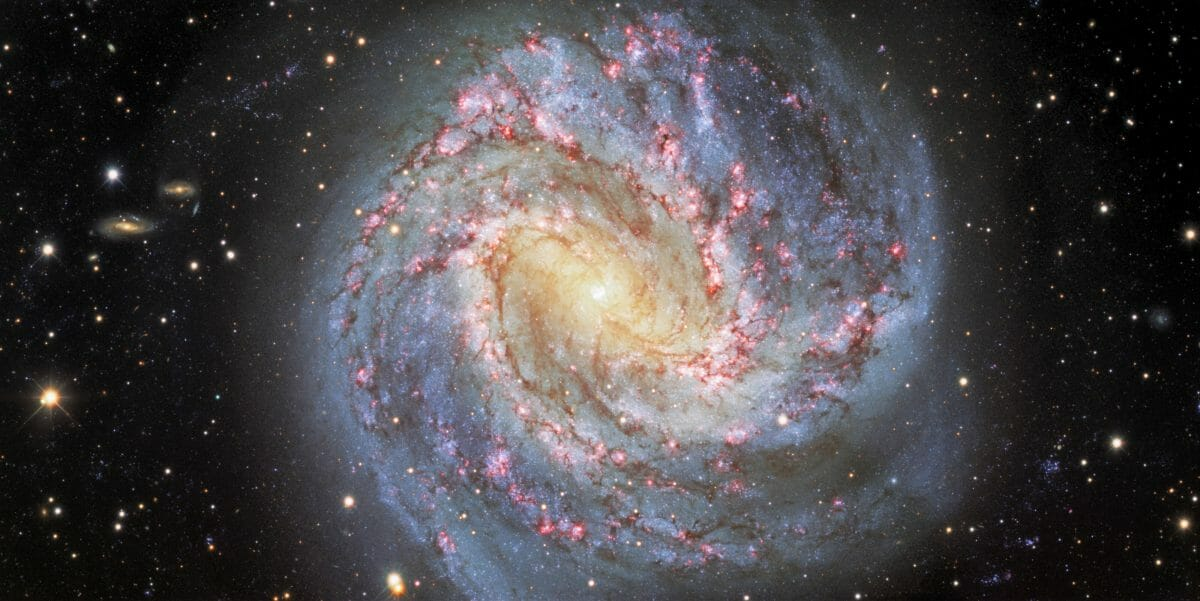
\includegraphics[width=1.0\linewidth]{m83.jpg}
\caption{\label{fig:m83}ここにキャプションが入る。M83は南の回転花火銀河とも呼ばれているらしい (Credit: CTIO/NOIRLab/DOE/NSF/AURA)。}
\end{figure}

ただし\LaTeX{}では挿入した位置にのまま画像が入るとは限らない。
また、画像と本文の間に1行空けないと\LaTeX{}変換時に画像をうまく認識してくれないので、画像の次の行は別段落として扱われる。
引用は「画像\ref{fig:m83}」のようにやる。
\subsection{コード}
\label{sec:orgc40e900}
\texttt{org-babel} を使ってPythonコードが挿入できる。
デフォルトでは\LaTeX{}に出力したときソースコードは全て \texttt{verbatim} で囲まれている。
そのためソースコードに装飾を施すためには工夫が必要になる。
\begin{itemize}
\item \href{https://orgmode.org/manual/Exporting-Code-Blocks.html}{Exporting Code Blocks (The Org Manual)}
\item \href{https://orgmode.org/manual/Results-of-Evaluation.html}{Results of Evaluation (The Org Manual)}
\end{itemize}

ソースコードをハイライトするパッケージとして \texttt{minted} が使える。
以下のコマンドで \texttt{minted} を使うことができる。
\begin{minted}[frame=lines,framesep=2mm,breaklines,bgcolor=bgcode]{common-lisp}
(setq org-latex-listings 'minted)
\end{minted}
\texttt{org-latex-minted-options} で \texttt{minted} 用の設定を記述することができる。
また \texttt{\textbackslash{}usepackage\{minted\}} を設定する必要がある。
\begin{itemize}
\item \href{https://qiita.com/clothoid/items/0a8f825ae19150fe5750}{emacs の org-latex-export-to-pdf 設定手順 \#Python - Qiita}
\end{itemize}

コードを書いたときのアウトプットは \texttt{:exports} 設定に依る。
デフォルトの \texttt{:exports} は \texttt{code} なので、Pythonコードは \texttt{python} 環境のときはコードがそのまま表示される。
\begin{minted}[frame=lines,framesep=2mm,breaklines,bgcolor=bgcode]{python}
import numpy as np
a = np.arange(10)
print(a)
\end{minted}

\texttt{ob-ipython} でも同様で、結果を実行していたとしても \texttt{:exports code} の場合は実行されない。
\begin{minted}[frame=lines,framesep=2mm,breaklines,bgcolor=bgcode]{ipython}
import numpy as np
np.arange(10)
\end{minted}

このとき \texttt{ob-ipython} を使って計算結果を走らせていたとしても、 \texttt{:results} に \texttt{drawer} が入っていると表示されないので注意する。
\begin{minted}[frame=lines,framesep=2mm,breaklines,bgcolor=bgcode]{ipython}
import numpy as np
np.arange(10)
\end{minted}

\begin{verbatim}
array([0, 1, 2, 3, 4, 5, 6, 7, 8, 9])
\end{verbatim}


出力パラメータが \texttt{:exports results} の場合にはコードが走った結果のみが表示される。
\texttt{:exports both} の場合にはコードと出力が表示される。
\texttt{:results raw} で \texttt{org} 上で出力していると、出力先には2重で表示されるので注意する。

また、あたりまえだが、\LaTeX{}やHTMLに出力するたびにコードが走るので動作が非常に遅くなって効率が悪い。
度々走らせる必要があるコード以外は先に出力しておいてそれを表示するだけの方が良い。
\texttt{:eval never-export} を設定するとエクスポート時に実行されなくなる。
\end{document}
